\section{Elektromagnet}
Elektromagneten er lavet til at holde bilen på banen. ved at aktivere elektromagneten sving burde den optimere bilens evne til at holde sig på banen, ved højre hastighed end udens elektromagnet.

\subsection{Kernemateriale}
En vigtig faktor i fremstilling af elektromagneter er materialet. Ud fra materialet bestemmes, elektromagnetens magnetiake evne, hvori materialets permabiliteten bestemmer hvor det kan lede et magnetisk felt. Permeabiliteten kan deles op i tre underemner, ferromagnetisk, paramagnetisk og diamagnetisk. \\
\begin{wrapfigure}{r}{0.5\textwidth}
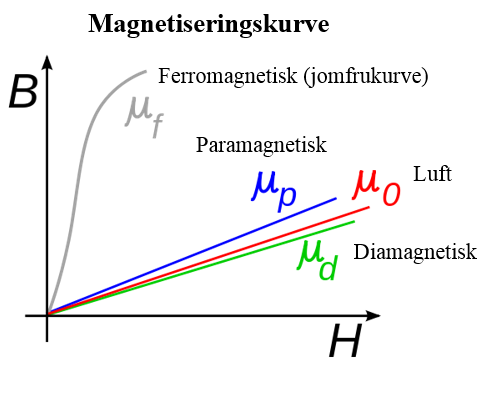
\includegraphics[scale=0.4]{./Graphics/Magnetiseringskurve}
\caption{Permeabilitete i forskellige materialer}
\label{Permeabilitet}
\end{wrapfigure}
I diamagnetiske materialer er magnetiseringen ekstremt lille og har en lineær BH-kurve. Ved paramagnetiske materialer er magnetiseringen ligeledes meget lille, men større end diamagnetiske materialer og ligeledes har materialet en lineær BH-kurve. Ferromagnetiske materialer har en stor magnetisering, den magnetiske effekt skyldes herved de uparede elektroner der forekommer i nogle metaller. Ferromagnetiske materialer har en logistisk stigende HB-kurve.\\
  \\
Ferromagnetisk materiale kan nu deles op i to undergrupper, blødt materiale og hårdt materiale. Blødt materiale er er karakteret ved høj permeabilitet, lille hysteresekurve med lille koerciv felt og lille kulstofindhold. Bløde materialer er ofte en legering af jern og silicium eller nikkel.\\
\begin{wrapfigure}{r}{0.5\textwidth}
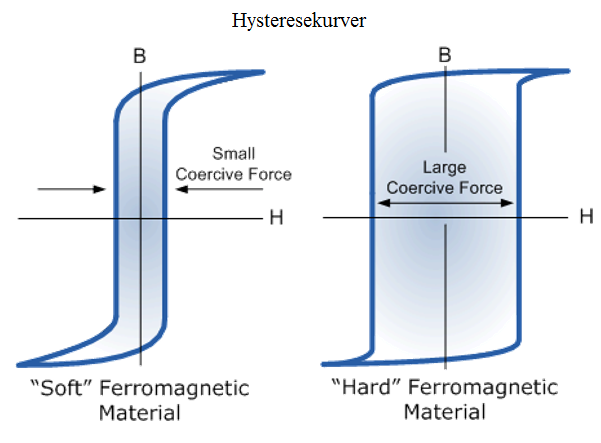
\includegraphics[scale=0.4]{./Graphics/Hysteresekurver}
\caption{Hysteresekurve på blødt og hårdt ferromagnetisk materiale}
\label{Hysteresekurve}
\end{wrapfigure}
Hårdt materiale er karakteriseret ved mindre permeabilitet end blødt materiale, bred hysteresekurve, stort koerciv felt og højt kulstofindhold. Hårde materialer er ofte en legering af jern med kulstof, aluminium eller wolfram. 

\subsection{Prøvemagnet}
Som udgangspunkt er kernematerialet blevet antaget til at være stål da materialet er ferromagnetisk og hårdt. hvis der skulle laves en korrekt undersøgelse at kernematerialet ville det kræve en længere og meget tidskræven undersøgelse, derfor har dette kun været en overvejelse. \\
Næste overvejelse har været placering og form af elektromagnet. der er tre steder elektromagneten kan placeres på bilen, der er foran, bagpå eller under bilen.\\
\begin{figure}
\center
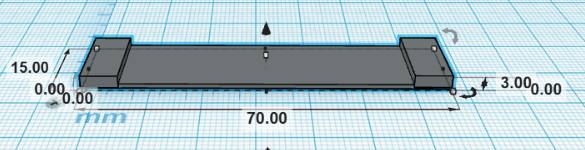
\includegraphics[scale=0.17]{./Graphics/Elektromagnet_2D}
\caption{Skabelon over elektromagneten med aktuelle mål}
\label{Elektromagnet_skabelon}
\end{figure}

Hverken trække eller skubbe elektromagneten er en effektiv løsning, det vil skabe uligevægt i bilen og flytte masse midtpunkt. ved en stærk elektomagnet vil man ændre friktions niveauet meget ved at have elektromagneten foran eller bagved, dvs. Hvis elektromagneten sidder bagpå vil der opstå meget friktion på baghjulene og mindre friktion på forhjulene.\\
Fluxspredning er en faktor der skal tages hensyn til når formen til elektromagneten laves, der vil altid være fluxspredning med formen kan være med til at reducere det betydligt. fluxlinjerne beværger sig fra nord til syd for fuldt udbytte af elektromagnet bør nord og syd pol befinde sig over skinnerne så fluxlinjerne løber med skinnerne. Hvis elektromagneten formes som en hestesko vil nord og syd pege ned mod skinnerne. for at undgå for meget fluxspredning bør luftgabet imellem nord og syd i hesteskoen være så stor som muligt, men da der er begrænset plads underbilen, kan lufgabet ikke blive særlig stort og en del kraft vil gå tabt i både fluxspredning og fluxfringing (se journal).\\

\begin{wrapfigure}{r}{0.5\textwidth}
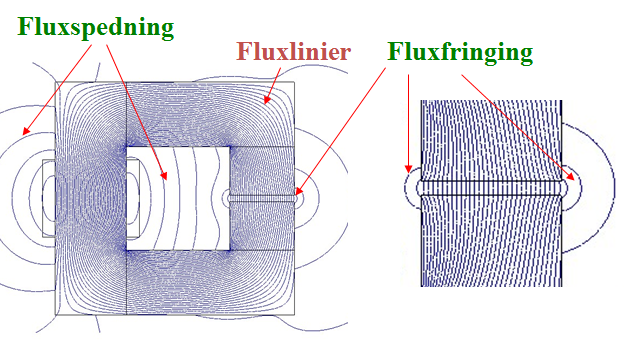
\includegraphics[scale=0.4]{./Graphics/Flux}
\caption{Flux, fluxfringing, fluxspredning}
\label{Flux}
\end{wrapfigure}

Nu da materialet er bestemt, placeringen og formen, skal antal vindinger bestemmes, da der er en maks bredde på pladsen under elektromagneten, vil der kun være plads til en 660 vindinger, før elektromagneten vil komme for tæt på banen, hvilket vil sige den ikke må komme tættere på end 2mm da bilen har affjedring og køre skævt i svingene. elektromagneten må ikke røre skinnerne da den enten vil gå i mætning eller kortslutte, så derfor er afstanden fra elektromagneten til skinnerne vigtigt.\\
\\
Test magneten er lavet ud fra forrige forhold og formlen for den magnetiske kraft i et luft gab (under idelle forhold) er givet ved:\\
\\
$F_{magn}(x)=-{\frac{B^{2}_{g}}{2\mu_{0}}}* {A_{j}}* (\frac{4x}{{\frac{l_{j}}{\mu_{r}}}+2x}-1) $
%$ {{\frac{4x}}{{frac{\l_{j}}{\mu_{r}}}}+2x}-1 $
\\
\\
Hvor $B_{g}$ er:
\\
\\
$ B_{g}(x)=\frac{\mu_{0}IN}{{\frac{l_{j}}{\mu_{r}}}+2x} $
\\
\\
Ud fra de overstående ligninger er kraften ideelt fundet til at være 1,309N. Virkeligt er den målt med en force sensor til at være 0,9367N. (henvis til journal) \\
Da 0,9367N er en meget lille kraft, bør de overvejes grundigt om elektromagneten vil blive en ulempe eller hjælp til bilen og hvor meget vil den lille kraft enlig kunne hjælpe med at forøge hastigheden i svingene. (henvis til peters afsnit)\\
